\documentclass[11pt,oneside,letterpaper]{article}

% graphicx package, useful for including eps and pdf graphics
\usepackage{graphicx}
\DeclareGraphicsExtensions{.pdf,.png,.jpg}

% basic packages
\usepackage{color} 
\usepackage{parskip}
\usepackage{float}

% text layout
\usepackage{geometry}
\geometry{textwidth=15cm} % 15.25cm for single-space, 16.25cm for double-space
\geometry{textheight=22cm} % 22cm for single-space, 22.5cm for double-space

% helps to keep figures from being orphaned on a page by themselves
\renewcommand{\topfraction}{0.85}
\renewcommand{\textfraction}{0.1}

% bold the 'Figure #' in the caption and separate it with a period
% Captions will be left justified
\usepackage[labelfont=bf,labelsep=period,font=small]{caption}

% review layout with double-spacing
%\usepackage{setspace} 
%\doublespacing
%\captionsetup{labelfont=bf,labelsep=period,font=doublespacing}

% cite package, to clean up citations in the main text. Do not remove.
\usepackage{cite}
%\renewcommand\citeleft{(}
%\renewcommand\citeright{)}
%\renewcommand\citeform[1]{\textsl{#1}}

% Remove brackets from numbering in list of References
\renewcommand\refname{\large References}
\makeatletter
\renewcommand{\@biblabel}[1]{\quad#1.}
\makeatother

\usepackage{authblk}
\renewcommand\Authands{ \& }
\renewcommand\Authfont{\normalsize \bf}
\renewcommand\Affilfont{\small \normalfont}
\makeatletter
\renewcommand\AB@affilsepx{, \protect\Affilfont}
\makeatother

% comments
\usepackage{ulem}
\definecolor{purple}{rgb}{0.459,0.109,0.538}
\def\tb#1#2{\sout{#1} \textcolor{purple}{#2}} 
\def\tbc#1{\textcolor{purple}{[#1]}}



%%% TITLE %%%
\title{\vspace{1.0cm} \LARGE \bf fluB}

\author[1]{Gytis Dudas}
\author[2]{Trevor Bedford}
\author[1]{Samantha Lycett}
\author[1,3]{Andrew Rambaut}

\affil[1]{Institute of Evolutionary Biology, University of Edinburgh, Edinburgh, UK}
\affil[2]{Vaccine and Infectious Disease Division, Fred Hutchinson Cancer Research Center, Seattle, WA, USA.}
\affil[3]{Fogarty International Center, National Institutes of Health, Bethesda, MD, USA.}

\date{\today}

\begin{document}
\maketitle

\begin{abstract}

Influenza B viruses are increasingly being recognized as major contributors to morbidity attributed to seasonal influenza. 
Currently circulating influenza B isolates are known to belong to two antigenically distinct lineages referred to as B/Victoria and B/Yamagata lineages on the basis of haemagglutinin inhibition (HI) assays. 
Frequent reassortment between the segments of these two lineages has been noted in the past \cite{lindstrom1999}, but the effects of these reassortments have not been investigated in much detail.

\end{abstract}

\pagebreak

\section*{Introduction}
Seasonal influenza causes an estimated 250,000 to 500,000 deaths annually and is comprised of three virus types (influenza A, B and C) co-circulating in humans, of which influenza A is considered to cause the majority of seasonal morbidity and mortality.
Though lacking the degree of antigenic diversity that influenza A viruses possess, influenza B viruses are increasingly being recognized as important human pathogens \cite{paul-glezen2013}.
Following the 2009 A/H1N1 pandemic, influenza B has increased in prevalence and in the 2012/2013 European season as many as 53\% of influenza sentinel surveillance samples tested positive for influenza B \cite{ECDC1213}. 

Like all members of \textit{Orthomyxoviridae}, influenza B viruses have segmented genomes, which allow viruses co-infecting the same cell to exchange segments (a process known as reassortment). 
Influenza A viruses are widely considered to be a major threat to human health worldwide due to the ability to cause pandemics in humans via reassortment of seasonal human and non-human influenza A strains. 
The only known persistent source of influenza B viruses are humans (and occasionaly seals \cite{osterhaus2000,bodewes2013}), thus limiting the virus's available antigenic reservoir. 
It has been suggested that influenza B viruses use a combination of reassortment and point mutations to generate antigenic diversity \cite{nerome1998,mccullers1999}.

Currently circulating influenza B viruses are comprised of two antigenically distinct lineages -- Victoria and Yamagata (referred to as Vic and Yam, respectively) -- named after two strains, B/Victoria/02/87 and B/Yamagata/16/88, which possess antigenically distinct haemagglutinin (HA) surface glycoproteins. 
The two HA lineages still co-circulate today and are thought to have emerged around 1983 \cite{rota1990}. 
All other influenza B segments also show a split around that time (our combined estimate across all segments place it \textit{circa} 1982.95 (95\% highest posterior density 1981.53--1984.21) figure \ref{TMRCAhpd}), although the numbers of strains falling on either side of the split are different due to reassortments following the initial split of Yam and Vic lineages in all segments and fixation of one or the other lineage in some segments.

%\begin{figure}[h]
%	\centering		
%	\includegraphics[width=0.95\textwidth]{figures/InfBtmrcaHPD}
%	\caption{\textbf{Provisional TMRCA plot.}}
%	\label{TMRCAhpd}
%\end{figure}

Previously, through the use of time-stamped phylogenetic trees, the reassortment history of major clades of influenza B has been reconstructed \cite{chen2008}, showing extensive and often complicated patterns of reassortment between all segments of influenza B viruses both between and within Vic and Yam lineages.

Another approach exists, however, whereby belonging to either the Victoria or Yamagata lineage in the tree of one segment can be used as a discrete trait in trees of other segments.
Reassortment events which result in the replacement of one segment lineage by another show up as changes in the discrete trait along a branch and allow the inference of parameters related to the subtree descended from the node displaying a changed trait (see Figure \ref{methodFig}).
Here, we use discrete traits to model inter-lineage reassortments between Victoria and Yamagata lineage segments in BEAST to look at lineage persistence times following reassortment events. 

We show that despite extensive reassortment, PB1, PB2 and HA segments of influenza B viruses still survive as Victoria and Yamagata lineages, which appear to be co-adapted to the point where virions which do not contain PB1, PB2 or HA segments derived entirely from either the Vic or the Yam lineage are selected against and, to the best of our knowledge, have not been sampled since 1996.
In other segments (PA, NP, NA, MP and NS) a single lineage has been fixed in the influenza B population: Yam for PA, NP, NA and MP and Vic for NS.

\begin{figure}[h]
 \centering		
	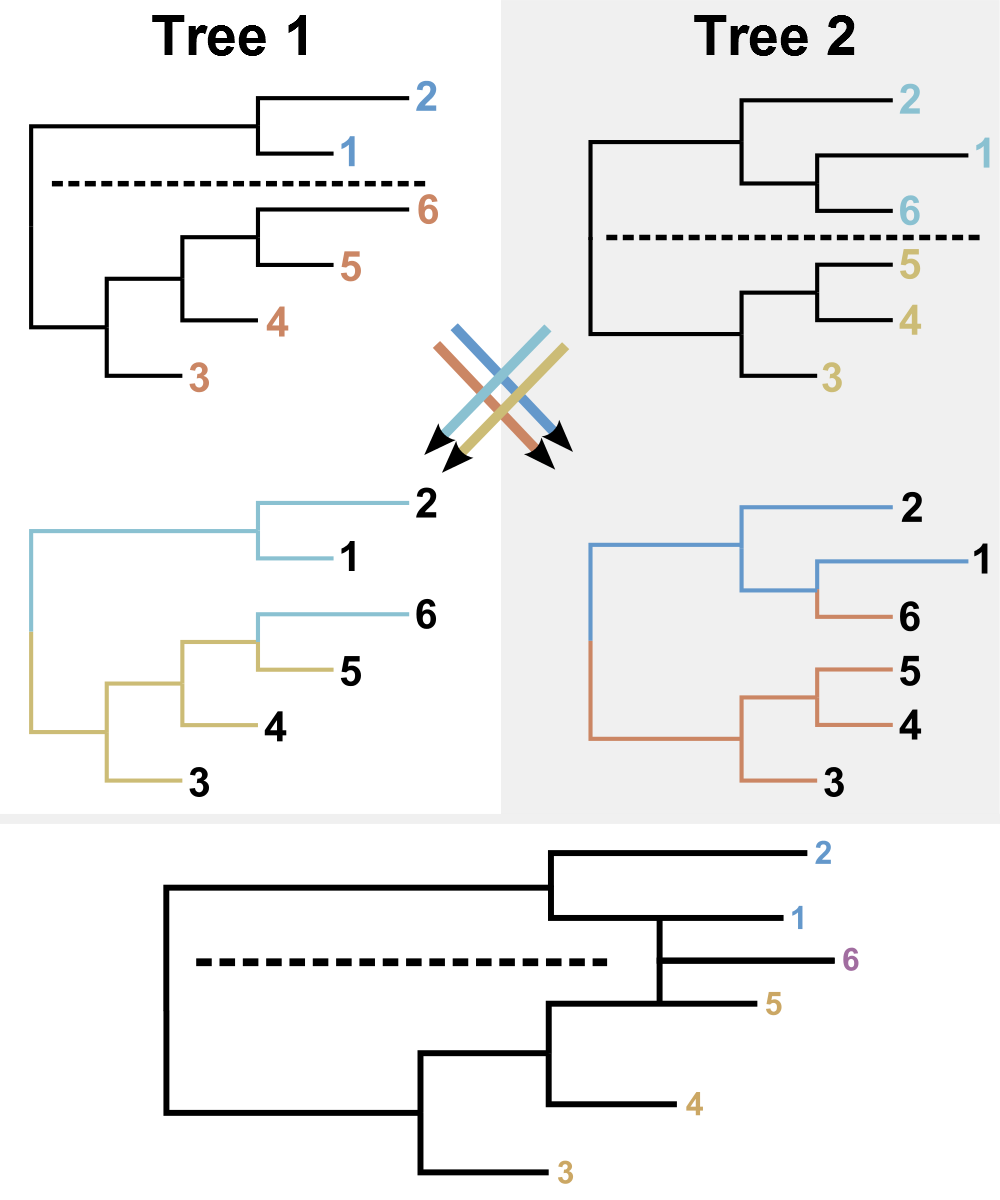
\includegraphics[width=0.45\textwidth]{figures/TreeFigure2}
	\caption{\textbf{Schematic depiction of method.}
We begin by assigning sequences falling on either side of a specified bifurcation within each segment tree to different lineages.
We then transfer lineage labels from one tree to the same tips in another tree.
Label switches thus indicate reassortment events that combine lineages falling on different sides of the bifurcation specified earlier.
In the example above tip number 6 is determined to be such a reassortant.}
	\label{methodFig}
\end{figure}

\section*{Methods}

\subsection*{Sequences and subtyping}
We compiled a dataset of 452 complete influenza B genomes from GISAID \cite{GISAID}. 
Each strain was assigned to a lineage (either Vic or Yam) in each segment by making maximum likelihood trees and looking whether it fell within the subtree containing B/Victoria/02/87 or B/Yamagata/16/88 sequences with the exception of the NS segment (B/Victoria/02/87 was a reassortant and possessed a Yam lineage NS \cite{lindstrom1999}), where B/Czechoslovakia/69/1990 was considered as being representative of Victoria lineage.

Each strain was thus assigned 8 lineages depending on the combination of lineages it belongs to in all trees (for example all segments except for NS in strain B/Victoria/02/87 belong to Vic lineage and can thus be represented as V,V,V,V,V,V,V,Y). 
Seven of these where then used as discrete states in each of the trees (e.g. PB1 tree had PB2, PA, HA, NP, NA, MP and NS as traits and V or Y as trait values) in BEAST \cite{drummond2012}.

\subsection*{Building trees}
Temporal phylogenies were recovered for each segment using the HKY model of nucleotide substitution, 3 codon partitions, robust counting \cite{obrien2009} and GMRF Bayesian skyride \cite{minin2008} as the demographic model over the course of an MCMC chain (3 parallel runs of 200 million states, sampling every 20000 steps).
In addition we used `relaxed' tips for 94 sequences (of which 93 only had year of isolation and 1 had only year and month of isolation) whereby tip dates would change and be estimated over the course of the MCMC chain (available in BEAST v1.7.4 \cite{drummond2012} via XML file editing as a date precision parameter).

We inferred the ancestral state of lineages in each segment by using discrete traits (asymmetric CTMC matrix with BSSVS \cite{lemey2009}). Because the posterior set of trees have branches labelled with the inferred lineage in all other segments, we can detect inter-lineage reassortments whenever a trait transition is observed (i.e. Y to V or V to Y, see Figure \ref{methodFig}) between a node and its descendant in any segment. 
In addition, by reconstructing the ancestral state of all other genomic segments jointly we can infer co-reassortment events when more than one trait transition occurs on the same node in a tree.

\subsection*{Measures of diversity}
We inferred the diversity of each segment over time by finding the oldest most recent common ancestor of all branches existing at yearly intervals, which places an upper boundary on the maximum amount of diversity existing at each time period.
In addition, we calculated mean pairwise TMRCA between branches inferred to be in virions possessing Vic and Yam lineage PB1, PB2 and HA.
This gave us an averaged measure of how much a particular segment reassorts with respect to PB1, PB2 and HA segments.
If Vic and Yam lineages of PB1, PB2 and HA segments were to be considered as being separate populations this measure would be equivalent to `between population' diversity.

We also calculated the total amount of evolutionary time each segment has spent in virions with entirely Vic, entirely Yam or mixed lineage PB1, PB2 and HA segments by taking the sum of branch lengths in each tree under different combinations of the PB1, PB2 and HA labels.
This gives a measure of how successful, over long periods of time, each particular PB1-PB2-HA constellation has been.

\subsection*{Tree to tree similarities}
In order to get a measure of tree to tree similarity we first extracted 1000 (sampling frequency roughly equal to 1 tree/180000 MCMC states) trees from the posterior distributions of trees of each segment.
Pairwise comparison between each pair of segments was performed by comparing trees at each MCMC state.

We express the similarity by referring to 3 descriptive statistics (sum, mean and standard deviation) of the distribution of TMRCA differences ($\Delta$TMRCA) between pairs of tips in the two trees.
These parameters are estimated for each pairing of trees at each MCMC state and provides us with 95\% highest posterior density intervals for those parameters, thus giving us the ability to test specific hypotheses regarding similarities between the trees of different segments.
Our approach exploits the branch scaling used by BEAST \cite{drummond2012}, since the trees are scaled in absolute time and therefore insensitive to variation in nucleotide substitution rates between segments, allowing for direct comparisons between TMRCAs in different trees.
If we are comparing TMRCAs of the same two tips in tree A and tree B we express it as $\frac{2\times [A:B]}{[A:A]+[B:B]}$, where [A:B] is $\Delta$TMRCA of a pair of tips between tree A and tree B and [A:A] is $\Delta$TMRCA between the same pair of tips between tree A and a replicate of tree A, to control for variability in tree topology stability over the course of the MCMC chain caused by differences in alignment lengths used to produce the trees.

We also attempted to calculate subtree prune and regraft (SPR) distances between trees using rSPR \cite{whidden2009,whidden2010,whidden2013}.
However, because the time taken to calculate the SPR distances depends on the SPR distances themselves, we find that SPR distance calculations over posterior sets of trees are impractical for all but the most similar trees.


\subsection*{Identifying linked sites in PB1, PB2 and HA segments}
We attempted to identify amino acid sites that exhibit linkage disequilibrium (LD) between PB1, PB2 and HA segments.
We chose the $\chi^{2}_{df}$ statistic \cite{zhao2005} for quantifying LD, as it is equal to the widely used \textit{r$^{2}$} LD statistic for biallelic loci, but also quantifies LD when there are more than two alleles per locus.

We also looked at amino acid sites which are different and fixed between sequences that were labelled as Victoria or Yamagata earlier and which possess entirely Victoria-derived or entirely Yamagata-derived PB1, PB2 and HA segments.
For the latter analysis we split our PB1, PB2 and HA amino acid alignments into temporal 5-year bins ranging from 1984 to 2013. 
By scanning Victoria and Yamagata alignments at each 5-year bin we can identify sites which are different and fixed between the two lineages and how the sites have evolved over the past 30 years.
This was done to control for sites in PB1, PB2 and HA proteins discovered by the LD analysis which, in addition to being more sensitive, might also be linked due to co-evolving sub-lineages within Vic and Yam lineages.

\section*{Results}

\subsection*{PA, NP, NA, MP and NS segments have periodically lost diversity}
The split of Vic and Yam lineages can be found in all segments.
Following the split of the two lineages, each segment could be assigned to either Vic or Yam lineage and inter-lineage reassortment events have yielded mixed-lineage genome constellations.
Some viruses with mixed-lineage genomes have become common ancestors to many later strains (i.e. the `trunk' of the phylogenetic tree) and the segment lineages involved so successful, as to become fixed within the influenza B population circulating today.

We find that Vic lineage PA, NP, NA and MP segments have gone extinct (i.e. no sequences from those lineages have been sampled in recent years see Figure \ref{lineageRatiosOverTime}), replaced entirely by the respective segments of Yam lineage in viruses bearing a Vic lineage HA.
Similarly, Vic lineage NS has become fixed in the viral population as well.
By looking at the oldest most recent common ancestor of all lineages existing within the tree of each segment at yearly timeslices (see Figure \ref{tmrcaOT}), it is clear that PA, NP, NA, MP and NS segments have undergone periodic losses of diversity, whereby sampled sequences trace their ancestry to increasingly more recent common ancestors.


\subsection*{PB1, PB2 and HA segments continue to circulate as two lineages and have not reassorted recently}
Unlike PA, NP, NA, MP and NS segments, which have periodically lost diversity, we find that PB1, PB2 and HA segments have continued to accumulate diversity since the initial split of Vic and Yam lineages (see Figure \ref{tmrcaOT}).
In addition, there is evidence to suggest that the numbers of sequences that belong to either Vic and Yam lineages of PB1, PB2 and HA segments have been sampled at a ratio close to 0.5 (see Figure \ref{lineageRatiosOverTime}), presumably due to the action of some form of balancing selection, possibly to maintain antigenic diversity.

By measuring the mean pairwise diversity between branches in each tree that were assigned either a Vic or Yam label in other segments, we look for reductions in diversity, which indicate that an inter-lineage reassortment event has taken place.
In example \ref{ARGexample}, if, over time slices, we measured mean pairwise distance between red and blue branches in tree 1, after they have been reciprocally labelled with each tip's position (with respect to some pre-defined bifurcation) in tree 2, we would find a drop in this measure, since the distance between tip 6 and tip 5 is now shorter and does not go through the root of the tree.
Thus, by measuring pairwise distances between differently labelled branches we get a sense of how panmictic different segments are with respect to each other.

If we repeat this procedure for all trees and focus on PB1, PB2 and HA lineage labels, we find that mean pairwise diversity between branches labelled as having for example, a PB1 segment of Vic or Yam lineage in PB2 and HA trees (and other combinations of the 3 trees and their labels), show small drops in diversity initially, but from the 1997 time slice onwards all branches labelled as Vic or Yam have a common ancestor at the root of the tree.
We also find evidence of co-reassortment in PB1, PB2 and HA segments: in Figure \ref{betweenDiversity} all three graphs become identical after 1997, indicating that the same PB1, PB2 and HA labels have been assigned to the same branches in trees of all other segments.
Our findings therefore suggest that a single configuration of Yam and Vic lineages of PB1, PB2 and HA segments has been preserved since the split of Vic and Yam lineages and have not reassorted with respect to each other, but rather have co-reassorted as a single unit, from 1997 onwards.

\begin{figure}
	\centering		
	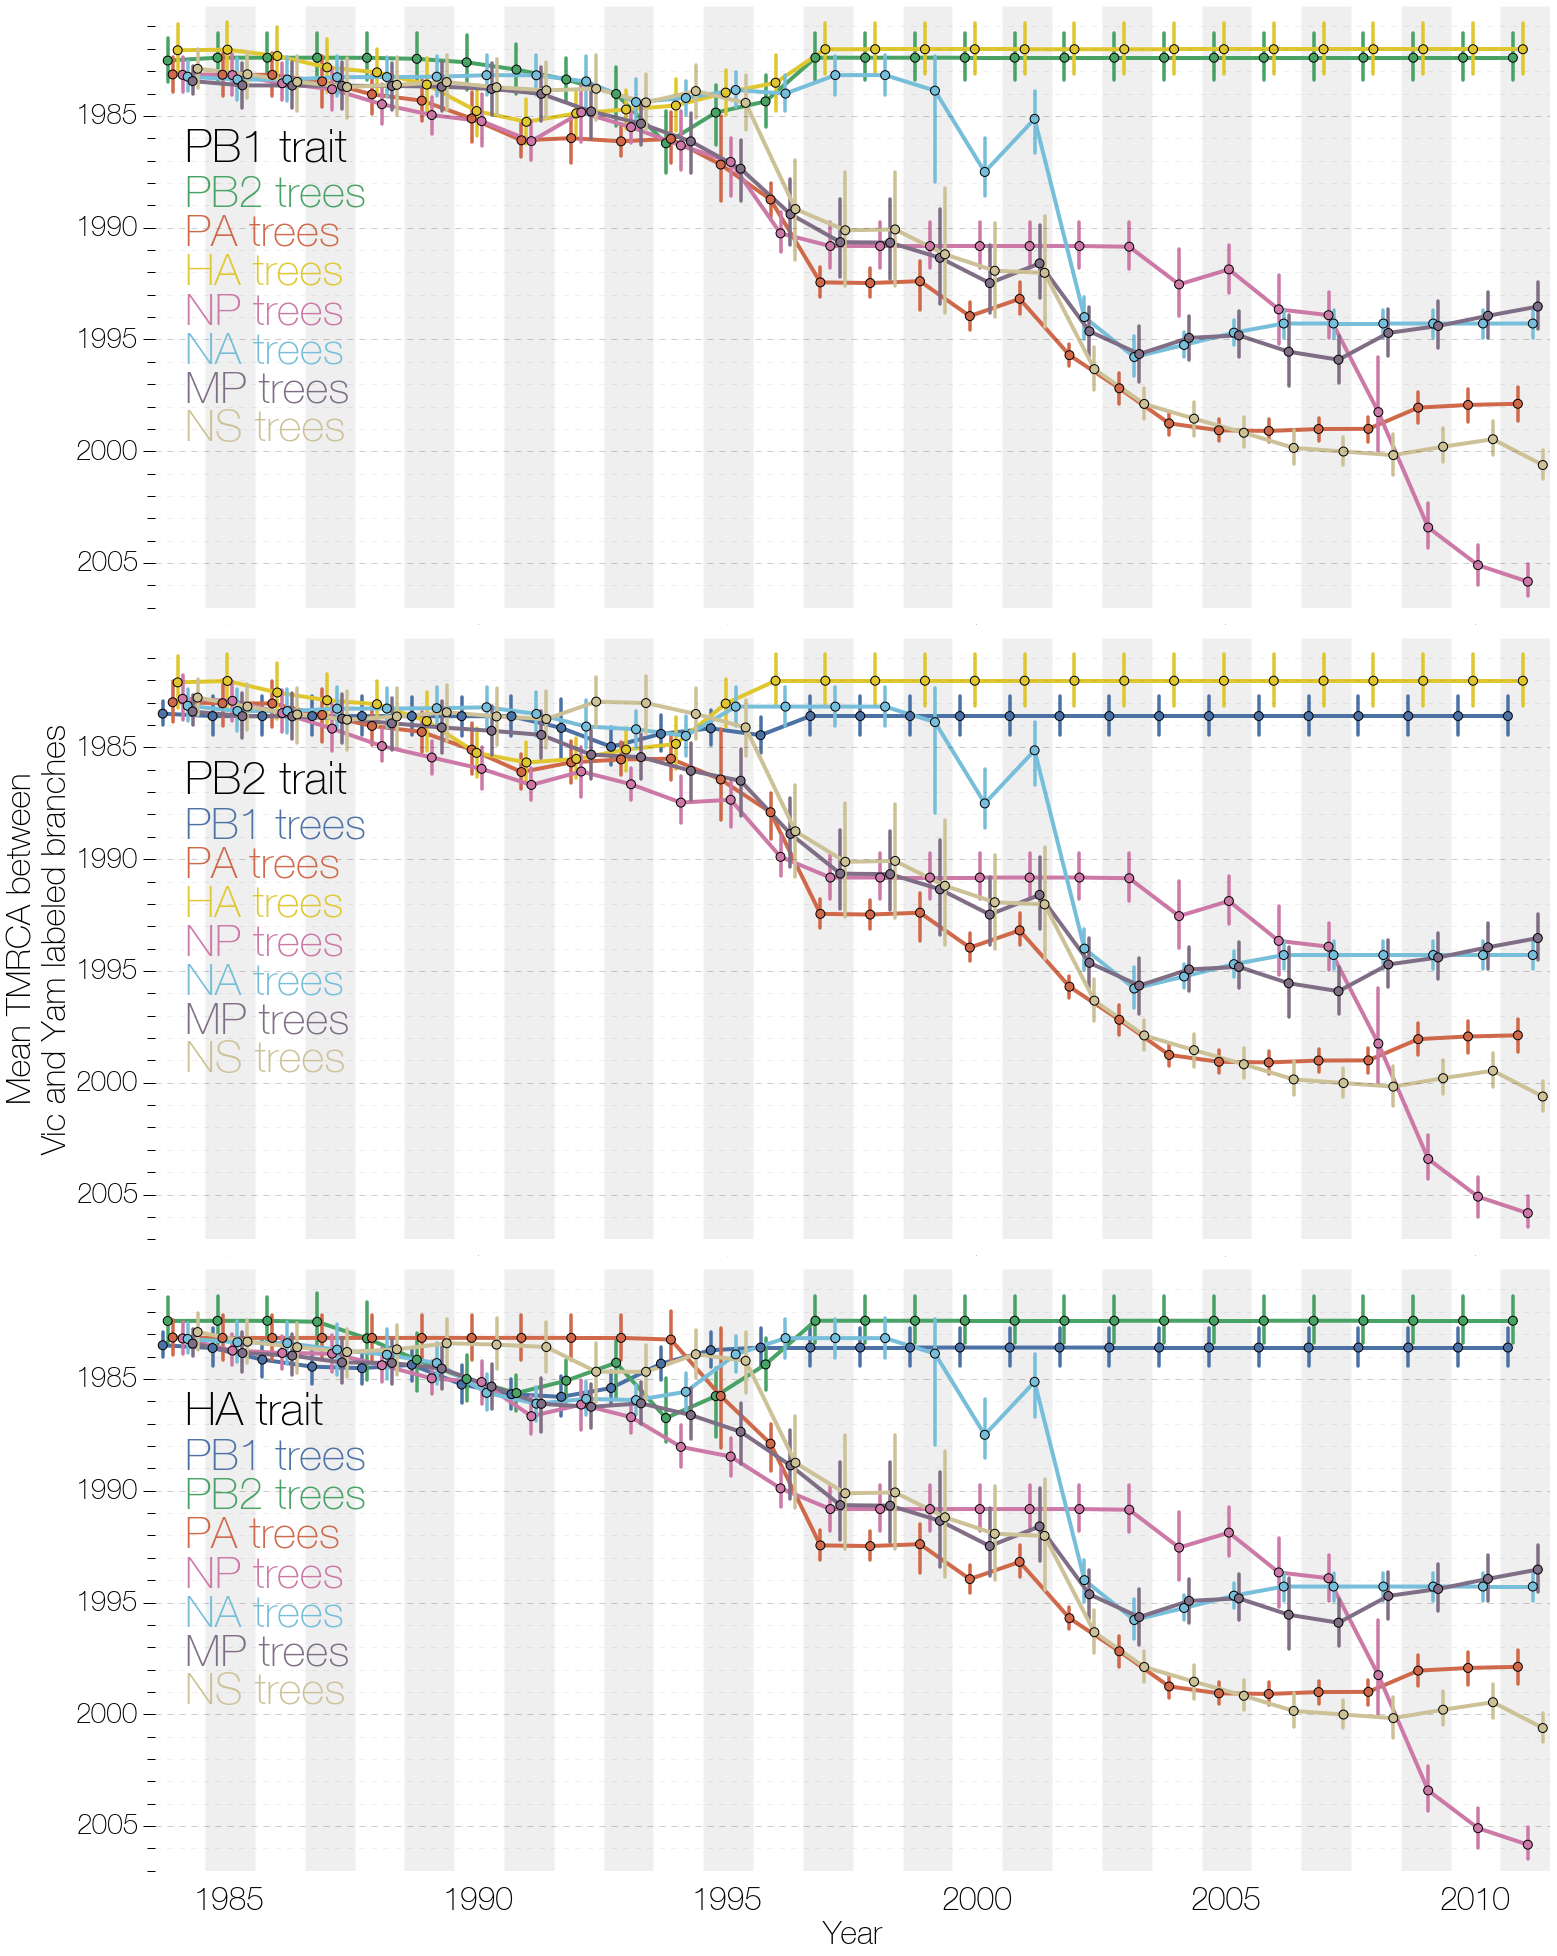
\includegraphics[width=0.95\textwidth]{figures/InfB_betweenDiversity.png}
	\caption{\textbf{Mean pairwise TMRCA between Vic and Yam branches under PB1, PB2 and HA label sets.}
PB1, PB2 and HA segment labels indicate that these segments show reciprocal preservation of diversity, which dates back to the split of Vic and Yam lineages.
All other segments show increasingly more recent TMRCAs between branches labelled as Vic and Yam in PB1, PB2 and HA label sets.}
	\label{betweenDiversity}
\end{figure}

\subsection*{Victoria and Yamagata lineages of PB1-PB2-HA are co-adapted segment complexes}
We find that PB1, PB2 and HA segments, in addition to not reassorting across the Vic-Yam lineage boundary recently, form co-reassorting segment complexes derived entirely of Vic or Yam lineage segments.
Figure \ref{stateTime} shows the sum of branch lengths which were labelled as having entirely Vic, entirely Yam or mixed-lineage PB1, PB2 and HA segments.

\begin{figure}[h]
	\centering		
	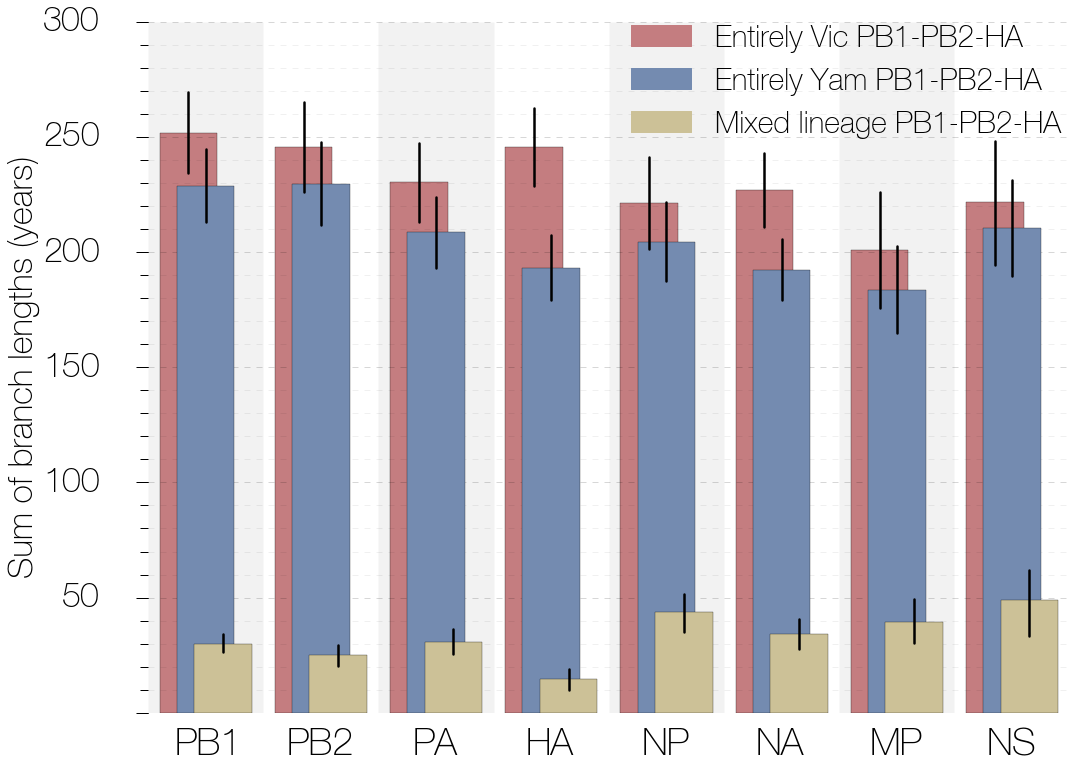
\includegraphics[width=0.95\textwidth]{figures/InfB_stateTime.png}
	\caption{\textbf{Amount of evolutionary time spent under different PB1-PB2-HA constellations.}
All segments have spent significantly more of their history with entirely Vic or entirely Yam-derived PB1-PB2-HA complexes.
(comment - based on 1 set of posteriors (comment - give numbers, HPDs)}
	\label{stateTime}
\end{figure}

Together with Figure \ref{betweenDiversity} it suggests that some inter-lineage reassortment has occured between PB1, PB2 and HA segments soon after the split of Vic and Yam lineages, but the resulting viruses were not fit and did not become the `trunk' of the tree.
Viruses bearing mixed-lineage PB1-PB2-HA complexes had the following constellations of PB1, PB2 and HA: VVY (B/Bankok/163/1990-like), YVV (B/Nanchang/630/1994-like) and YVY (B/New York/24/1993-like).
We do not show results for other lineage labels as none of them show this pattern of reciprocally preserved diversity with any other segment.

\subsection*{Other segments evolve with considerable independence}
The reconstructed evolution of Victoria and Yamagata lineages of all segments reveals a considerable degree of autonomy.
For example, of all the Yamagata lineage segments that were reassorted into Victoria lineage PB1-PB2-HA background giving rise to B/Hong Kong/330/2001-like viruses, most segments went extinct following later reassortments, save for NP, which continued circulating until, at the latest, 2011.
A more dramatic example can be found in the NS segment, where the Vic lineage had been fixed in the population after reassorting into an otherwise entirely Yam-derived genome constellation and then reassorted back into a Vic lineage PB1-PB2-HA background, replacing the NS lineage that was present there. 

\begin{figure}[h]
	\centering		
	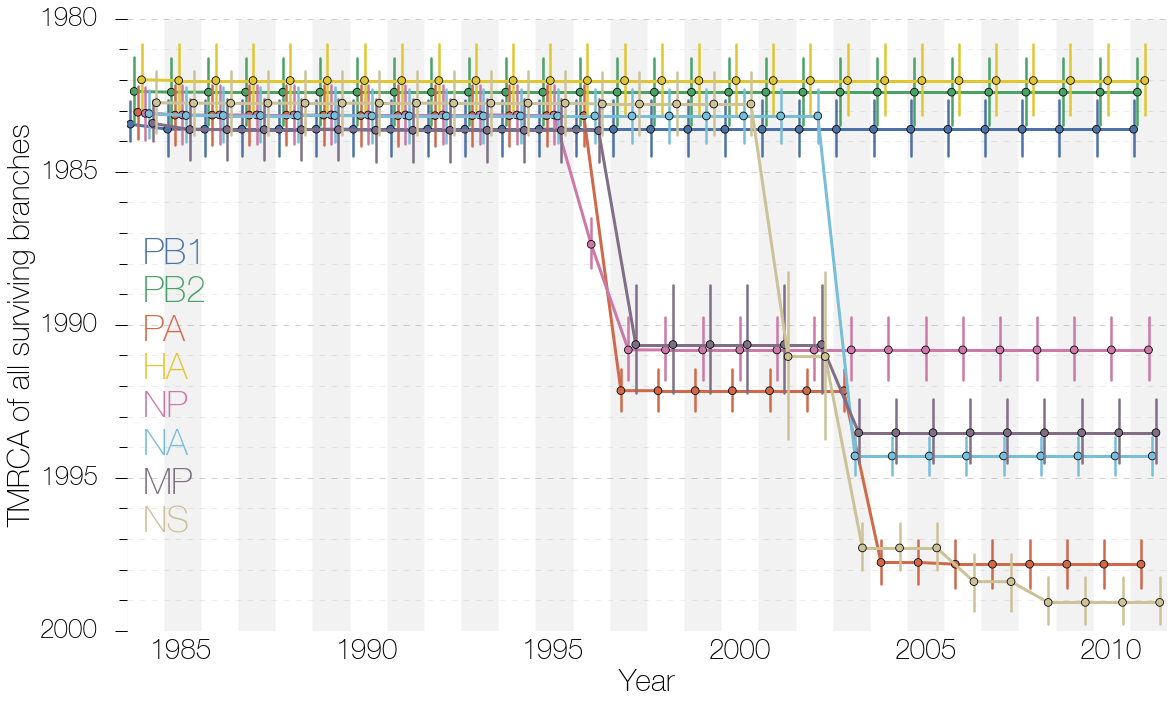
\includegraphics[width=0.95\textwidth]{figures/InfB_tmrcaOT_lines.png}
	\caption{\textbf{Oldest TMRCA of all surviving lineages over time.}
PA, NP, NA, MP and NS segments of influenza B viruses show periodic losses of diversity, indicating lineage turn over.
PB1, PB2 and HA segments, on the other hand, maintain the diversity dating back to the initial split of Vic and Yam lineages.}
	\label{tmrcaOT}
\end{figure}

(comment - need higher resolution for lineage ratios figure or switch to vector graphics)
\begin{figure}[h]
	\centering	
	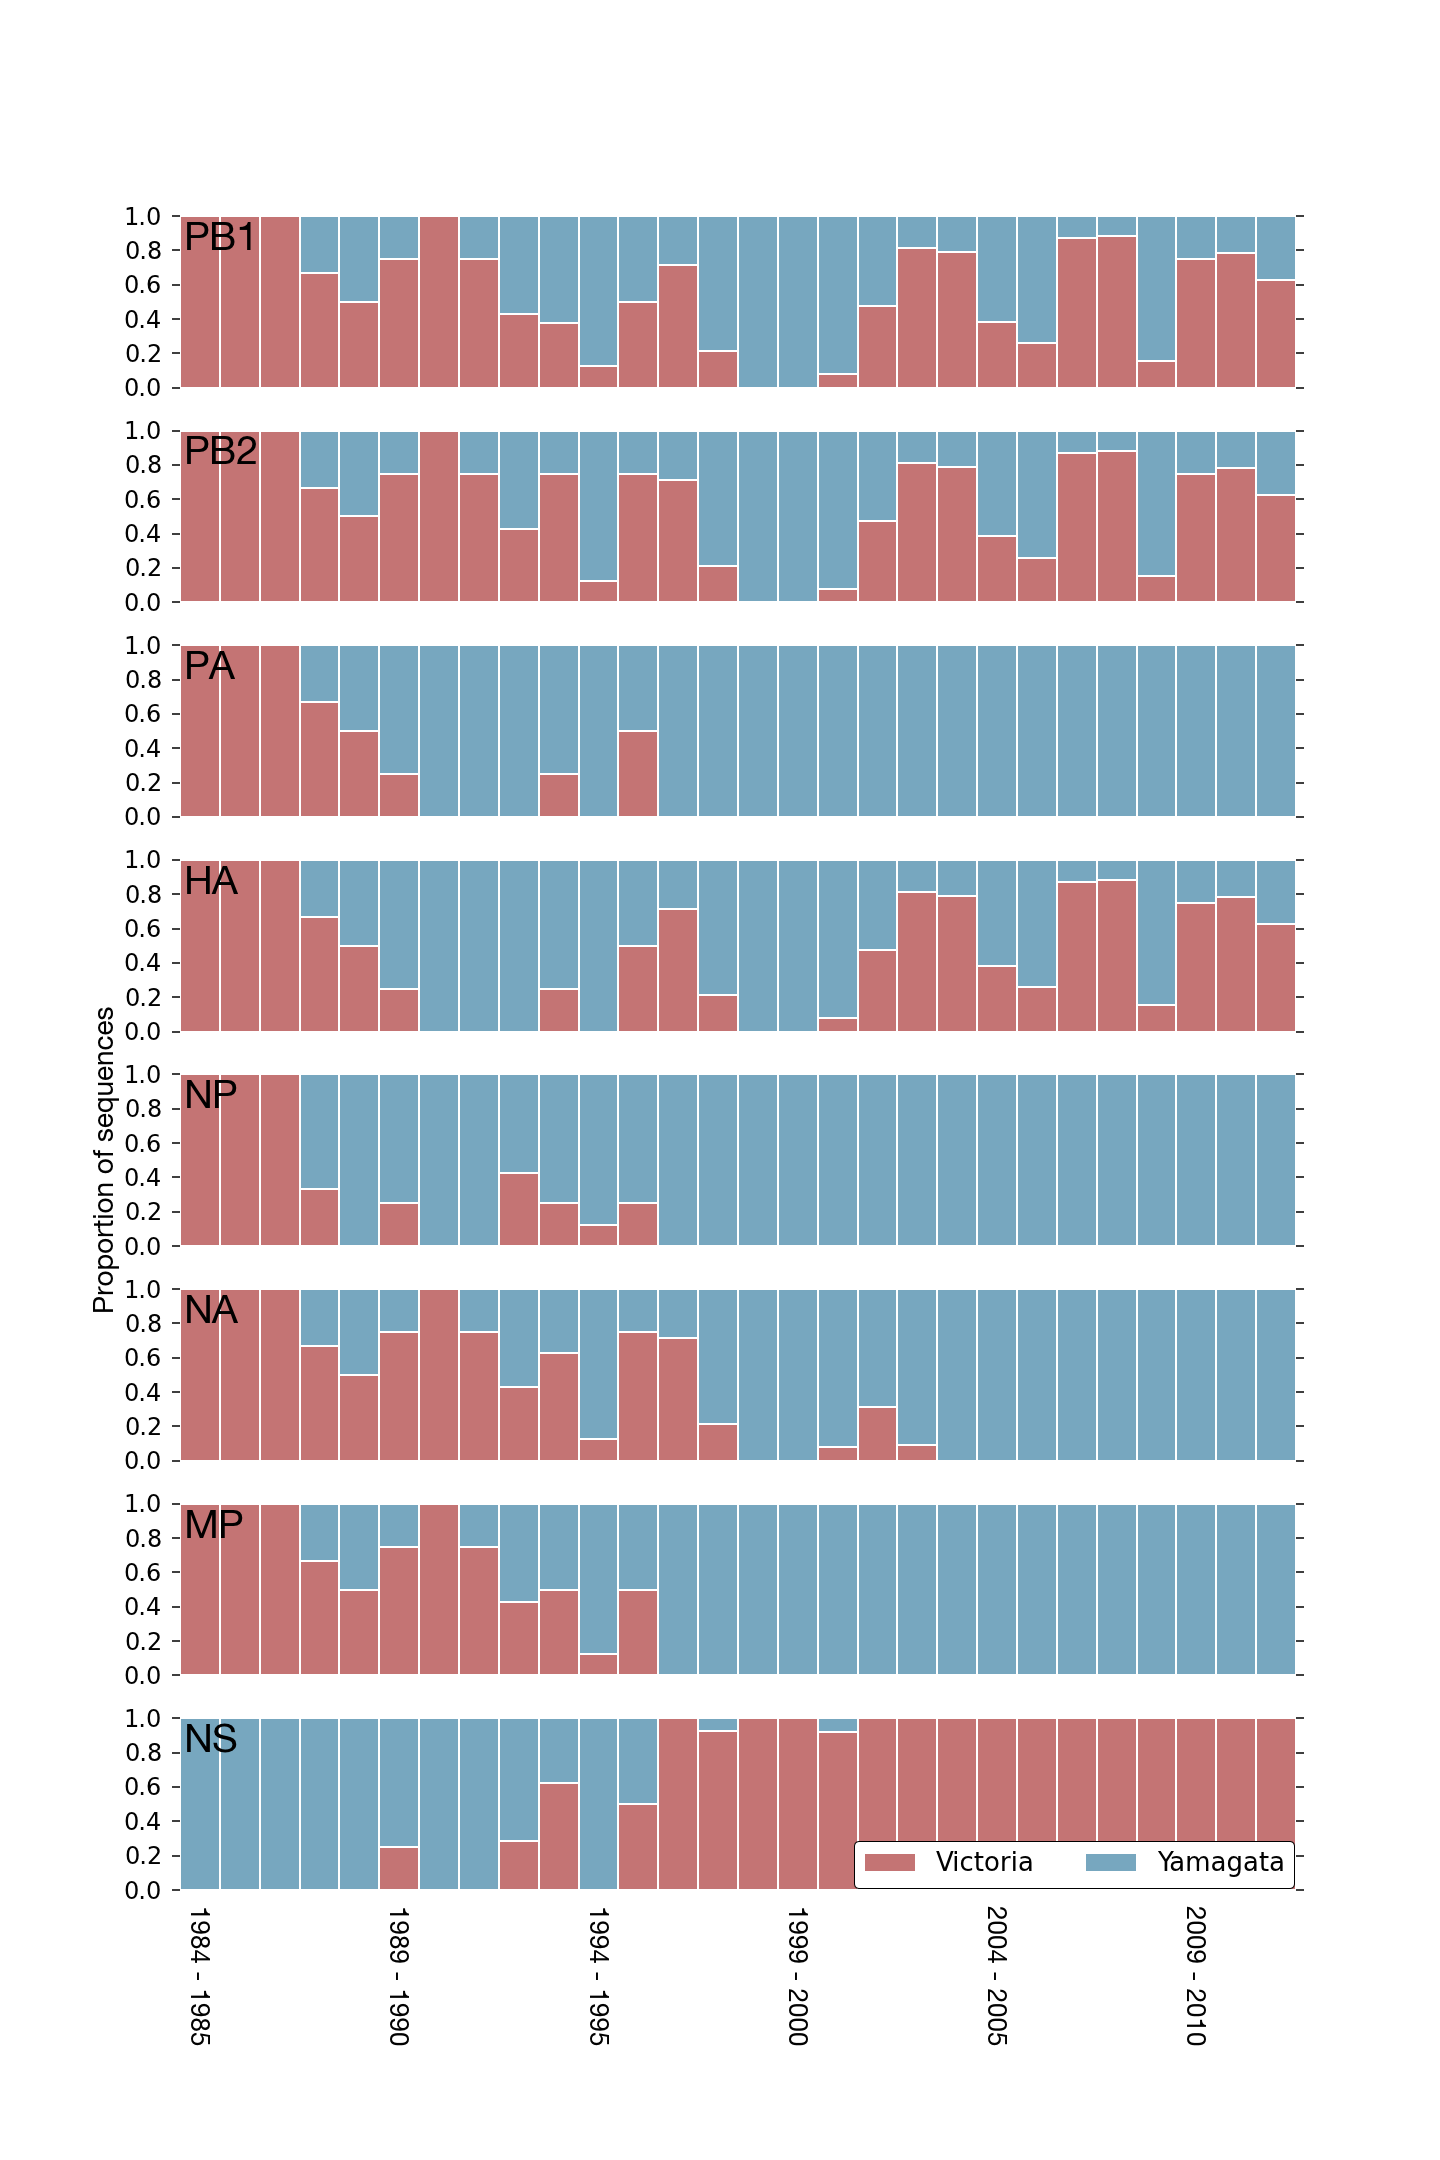
\includegraphics[width=0.75\textwidth]	{figures/InfB_LineageRatiosOverTime.png}
	\caption{\textbf{Ratio of lineages in the dataset.}}
	\label{lineageRatiosOverTime}
\end{figure}

\begin{table}[h]
	\centering
	\label{stateTimeTable}
	\caption{Amount of evolutionary time spent under different PB1-PB2-HA constellations.
All segments have spent significantly more of their history with entirely Vic or entirely Yam-derived PB1-PB2-HA complexes.}
	\makebox[\textwidth][c]{
	\begin{tabular}{ c | c c c c } 
	\hline
	Segment						&	PB1				&	PB2				&	PA				&	HA					\\ \hline	
	Victoria mean 95\% HPDs		&	\textbf{251.21}	&	\textbf{245.13}	&	\textbf{230.51} 	&	\textbf{245.46} 		\\
								&	234.43--270.60	&	 226.25--264.23	&	212.94--247.24	&	228.94--262.99 		\\
	Yamagata mean 95\% HPDs		&	\textbf{228.66} 	&	\textbf{229.65} 	&	\textbf{208.38} 	&	\textbf{192.82} 	 	\\
								&	212.94--244.51	&	211.80--247.79	&	193.28--224.65	&	179.30--207.69		\\
	Mixed-lineage mean 95\% HPDs	&	\textbf{30.06} 		&	\textbf{25.06} 		&	\textbf{30.90} 		&	\textbf{14.45} 		 	\\
								&	26.46--34.16		&	20.54--29.69		&	25.22--36.13		&	10.14--18.80			\\
	\hline
	Segment							&	NP				&	NA				&	MP				&	NS				\\ \hline	
	Victoria mean 95\% HPDs			&	\textbf{220.60} 	&	\textbf{226.73} 	&	\textbf{202.38} 	&	\textbf{222.23}	\\
									&	201.65--241.03	&	210.91--242.12	&	176.77--227.67	&	193.31--249.61 	\\
	Yamagata mean 95\% HPDs		 	&	\textbf{204.18} 	&	\textbf{192.27} 	&	\textbf{184.13} 	&	\textbf{210.93} 	\\
									&	188.68--221.73	&	179.28--205.74	&	165.97--204.10	&	190.02--231.61	\\
	Mixed-lineage mean 95\% HPDs 		&	\textbf{43.66}		&	\textbf{34.05} 		&	\textbf{39.41} 		&	\textbf{49.36} 		\\
									&	34.67--50.86		&	27.50--40.90		&	29.80---48.90	&	33.49--62.62		\\

	\end{tabular}	
	}
\end{table}

\subsection*{Co-adaptation candidate sites do not fall within intuitive regions of PB1, PB2 and HA proteins}
We find that amongst the pairs of sites exhibiting the highest $\chi^{2}_{df}$ statistics none fall within the regions previously described as forming the contacts between PB1 and PB2 proteins of the influenza A polymerase.
Linkage disequilibrium analysis of the HA segment shows that as many as 11-12\% of the amino acid sites in HA exhibit high linkage disequilibrium with respect to PB1 and PB2 segments (compared to 6-7\% in PB1 and PB2).
This probably reflects the independent accumulation of advantageous amino acid substitutions within Victoria and Yamagata lineages and sub-clades.
In fact all amino acid sites in the HA segment exhibiting high linkage disequilibrium with sites on PB1 and PB2 segments are found within the HA1 region of HA.




\section*{Discussion}

\subsection*{Limitations of current study}
The methods used in this paper have limited power to detect reassortments, since lineages have been fixed over time and thus all viruses eventually come to bear either Vic or Yam lineage PA, NP, NA, MP and NS segments.
We can also only detect reassortment events where a lineage has switched from Vic to Yam or \textit{vice versa}, but not when a lineage has switched from a Yam lineage to another Yam lineage, which has occurred in the past (e.g. the reassortment events giving rise to B/California/NHRC0001/2006-like and B/Brisbane/33/2008-like viruses, which involved a Vic lineage PB1-PB2-HA complex reassorting with NP of Yamagata lineage is only visible in the NP tree, since all viruses in our dataset from 1995 onwards, including Vic PB1-PB2-HA complex-bearing ones, already had a Yamagata lineage-derived NP).
However, this study focuses on PB1, PB2 and HA segments, all of which have survived as two lineages up to this day and thus are more informative for inferring reassortments.

\subsection*{PB1-PB2-HA co-adaptation has evolved over time}
Our findings suggest that PB1, PB2 and HA segments of Vic and Yam lineages represent co-adapted co-reassorting segment complexes.
Previous studies have suggested similarities between the evolution of PB1, PB2 and HA segments of influenza B viruses \cite{hiromoto2000,lindstrom1999}, based on topology similarities between phylogenetic trees of the three segments, albeit the trees used in those studies contained limited numbers of sequences sampled somewhat close in time to the split of Victoria and Yamagata lineages.
Despite the apparent similarities between PB1, PB2 and HA trees, we have detected at least 3 genome constellations having mixed-lineage PB1-PB2-HA sampled early in the first decade of the split between Vic and Yam lineages, when, presumably, Vic and Yam lineages of PB1, PB2 and HA segments were still similar at the amino acid level to produce viable, though presumably unfit, influenza B viruses.

Our results also suggested that all segments have spent very little evolutionary time in the same virions as the 3 mixed-lineage PB1-PB2-HA constellations, compared to either entirely Yam PB1-PB2-HA or entirely Vic PB1-PB2-HA bearing viruses.
We interpret lack of reassortment within the PB1-PB2-HA complex across the lineage boundary in recent times as evidence of a considerable degree of co-dependence within the Vic and Yam PB1-PB2-HA lineages, whereby recent reassortants bearing mixed-lineage PB1-PB2-HA complexes are inviable or unsampled by surveillance due to being outcompeted by viruses with pure-lineage PB1-PB2-HA complexes.

\subsection*{Potential causes of co-dependence between PB1-PB2-HA}
Previous studies have investigated possible co-dependence patterns between segments of influenza B viruses, by focusing on segments which would be expected to be co-adapted, e.g. PB1-PB2-PA and HA-NA \cite{mccullers2004}.
Though it would be easy to explain co-adaptation between the aforementioned segments by referring to their functional roles (e.g. PB1-PB2-PA form the polymerase heterotrimer and HA-NA have antagonistic activities), our findings suggest a counter-intuitive relationship between PB1, PB2 and HA segments.

It is clear that PB1-PB2-HA segments of Vic and Yam lineages do not preferentially reassort together, because there have been at least 3 sampled mixed-lineage PB1-PB2-HA complex constellations, which did not become fixed in the population and recent evidence suggests that, at least in influenza A, reassortment between segments differing by a single synonymous difference is highly efficient \cite{marshall2013}.
In the absence of clear functional explanations for why PB1, PB2 and HA should be co-adapted we suggest several alternatives.

Many studies have noted a possible link between the HA, NA and PB1 segments of influenza A viruses \cite{bergeron2010,fulvini2011}.
Early influenza A vaccines were derived by infecting chicken eggs with an egg-adapted strain and a seasonal human isolate in the presence of antisera raised against the HA and NA proteins of the egg-adapted strain, thus selecting for reassortants which were egg-adapted (\textit{i.e.} had internal segments derived from the egg-adapted strain) but possessed the HA and NA segments of the seasonal strain.
However, in addition to producing reassortants with HA-NA derived from the seasonal strain, as intended, the second most frequent class of reassortants produced using this methods were those with PB1, HA and NA derived from seasonal strains \cite{bergeron2010,fulvini2011}.

Recent experiments have suggested that the presence or absence of a `foreign' PB1 segment can have dramatic effects on HA concentration on the surface of virions and total virion production \cite{cobbin2013}.
Additional evidence for a relationship between PB1 and HA segments in influenza A viruses is given by previous influenza pandemics, which were caused by avian-human influenza A virus reassortants.
It has been established that at least for the 1957 and the 1968 influenza pandemics, caused by A/H2N2 and A/H3N2 subtypes, respectively, the viruses responsible were reassortants possessing PB1 and HA segments (and in the case of A/H2N2, NA as well) derived from avian influenza A viruses \cite{kawaoka1989}.

Another possibility is the action of balancing selection in preserving the diversity in one segment, whilst the other segments hitchhike along.
A good candidate for this would be HA, as it is now the sole bearer of antigenic diversity within the influenza B population (the Vic lineage NA segment having gone extinct), until the Yam lineage NA segment under Vic PB1-PB2-HA recovers sufficient antigenic diversity.
Previous research has found that avian influenza A virus HA and NA segments, which are the primary vehicles of antigenicity, exhibit vast diversity when compared to `internal segments', which show much more recent TMRCAs and less variability at the amino acid level \cite{chen2006,obenauer2006}.
It is also possible that Vic and Yam lineages of PB1, PB2 and HA segments have simply drifted away from each other, without any one segment being the driver of diversity preservation in PB1, PB2 and HA segments.
This process, termed mutation-driven co-evolution \cite{presgraves2010}, has been suggested to be the cause of hybrid dysfunction in hybrids of \textit{Saccharomyces cerevisiae} and \textit{Saccharomyces bayanus} \cite{lee2008}.

\subsection*{The future of influenza B viruses}
We see two potential paths of evolution for influenza B viruses.
More segments could be recruited into co-adapted segment complexes (PB1, PB2 and HA segments having started this first), as part of a speciation process, until all circulating influenza B viruses possess genomes with segments firmly associated with either the Vic or Yam lineage PB1-PB2-HA complex which could be referred to as belonging to either `new Victoria' or `new Yamagata' lineages.

This may seem to be the case in Figure \ref{tmrcaOT} where the NP segment, exhibiting the fourth oldest TMRCA by 2011, looks like it might begin co-evolving with the PB1-PB2-HA complexes. 
However, the continuous measure of diversity between Vic and Yam lineages of PB1, PB2 and HA segments in Figure \ref{betweenDiversity} show that the NP segment is skewed towards very recent TMRCAs, suggesting that a large number of recent isolates are products of recent reassortment between the NP segment and PB1-PB2-HA complexes (in fact, this is due to viruses possessing B/Brisbane/33/2008-like genome constellations, which comprise a large part of recently isolated influenza B virus strains).
The other alternative is continued reassortment of all non-PB1-PB2-HA segments between Vic and Yam PB1-PB2-HA complexes, or even extinction of one or the other lineage of the PB1-PB2-HA complex.

Given the relatively recent explosion of sequence data available for influenza B, it is difficult to say whether such two-lineage dynamics have not occurred in the history of influenza B viruses.
If the influenza B population is on its way to speciation we expect that over time inter-lineage reassortment frequency should decrease, as more and more segment lineages get recruited into co-adapted segment complexes.

On the other hand, influenza B viruses might continue co-circulating as two PB1-PB2-HA lineages exchanging non-PB1-PB2-HA segments, with reassortment frequency being roughly constant.
Seeing how rarely influenza B viruses reassort across the Vic-Yam lineage boundary, the timescale for finding out which of the aforementioned scenarios, if any, are under way, is impractical at best.

\subsection*{Predictions}
Using previously developed plasmid systems \cite{hoffmann2002} it would be possible to create artificial reassortants, combining Vic and Yam lineages of PB1, PB2 and HA segments into mixed-lineage PB1-PB2-HA complexes.
We predict that artificially produced viruses with mixed-lineage PB1-PB2-HA complexes will have reduced fitness when compared to viruses with pure-lineage (\textit{i.e.} entirely Vic or entirely Yam) PB1-PB2-HA complexes.
In addition, we expect the relationship between Vic and Yam lineage PB1, PB2 and HA segments to be dependent on date of segment isolation, as viruses with mixed-lineage PB1-PB2-HA complexes isolated earlier should perform better than viruses with PB1-PB2-HA segments isolated more recently.

However, we also see that epistatic effects might interfere with fitness measurements, if for example non-PB1-PB2-HA segments are also temporally mismatched.
Ideally, the co-adaptation would be easier to understand by referring to the structures of PB1 and PB2 proteins, as the link between these would be intuitive.
We have identified amino acid sites which are linked between PB1, PB2 and HA proteins of Victoria and Yamagata lineages, but we find very few sites on PB1 and PB2 proteins that fall within the regions that form contacts within the influenza B polymerase heterotrimer, suggesting more subtle roles for sites we have identified.

\subsection*{Implications for influenza B virus control and prevention}
It is our hope that understanding the mechanism(s) underlying the links between Vic and Yam lineage PB1-PB2-HA complexes might suggest a more varied approach to both influenza B surveillance and control.
For one, our findings suggest that viruses bearing mixed-lineage PB1-PB2-HA complexes, if unveiled by surveillance, are unlikely to contribute to future influenza B evolution.
Similarly, in the absence of sequence data, it should be possible to predict the lineage of PB1, PB2 and HA segments of influenza B viruses by sequencing only one of those segments.

It remains to be seen whether equivalent or similar links exist between segments of influenza A viruses, which present a much greater threat to human health worldwide than influenza B viruses.
By discovering the underlying mechanism by which PB1, PB2 and HA are co-adapted might reveal potential targets for new classes of antiviral drugs.

\section*{Conclusions}
In this study we have investigated the patterns of reassortment amongst two influenza B virus segment lineages and found preserved diversity and consistent co-reassortment of 3 segments: PB1, PB2 and HA.
Our findings reveal that Vic and Yam PB1, PB2 and HA segments co-associate amongst themselves with segments of their own lineage, thus resulting in an entirely Vic-lineage-derived PB1-PB2-HA segment complex and an entirely Yam-lineage-derived PB1-PB2-HA segment complex that co-circulate within the influenza B virus population, occasionally exchanging non-PB1-PB2-HA segments.
Though we detect strains with mixed-lineage PB1-PB2-HA complexes early after the split between Vic and Yam lineages, we find that they have performed poorly and have circulated for short amounts of evolutionary time when compared to viruses with `pure' lineage PB1-PB2-HA complexes.

We argue that this is evidence for a selectively maintained relationship between PB1-PB2-HA complex of Vic and Yam lineages and not due to biased reassortment.
In addition, the close timing of these mixed-lineage PB1-PB2-HA reassortants close to the split of Vic and Yam lineages suggests that the relationship between each lineage's PB1-PB2-HA complexes have developed over time and in their current state reassortant viruses with mixed-lineage PB1-PB2-HA complexes are undetected by surveillance due to either poor fitness or inviability.



%\begin{figure}[h]
%	\centering		
%	\includegraphics[width=0.95\textwidth]{figures/InfB_TMRCAOverTime}
%	\caption{\textbf{Provisional TMRCA over time plot.}}
%\end{figure}


\bibliographystyle{pnas}
\bibliography{fluB}
\end{document}
